%%%%%%%%%%%%%%%%%%%%%%%%%%%%%%%%%%%%%%%%%%%%%%%%%%%%%%%%%%
\begin{frame}
\frametitle{Spark Applications: The Big Picture}
%%%%%%%%%%%%%%%%%%%%%%%%%%%%%%%%%%%%%%%%%%%%%%%%%%%%%%%%%%
\begin{itemize}
	\item There are two ways to manipulate data in Spark
	\begin{itemize}
		\item Use the interactive shell, \textit{i.e.,} the REPL
		\item Write standalone applications, \textit{i.e.,} driver programs
	\end{itemize}
\end{itemize}

	\begin{figure}[h]
	  \centering
	  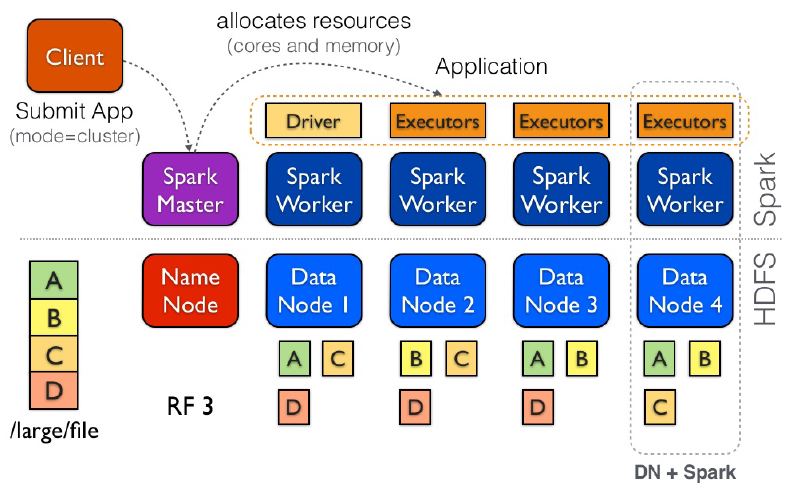
\includegraphics[scale=0.33]{./Figures/spark_app_overview}
	  \label{fig:spark_app_overview}
	\end{figure}
\end{frame}

%%%%%%%%%%%%%%%%%%%%%%%%%%%%%%%%%%%%%%%%%%%%%%%%%%%%%%%%%%
\frame {\frametitle{Spark Components: details}
%%%%%%%%%%%%%%%%%%%%%%%%%%%%%%%%%%%%%%%%%%%%%%%%%%%%%%%%%%
\begin{figure}[h]
  \centering
  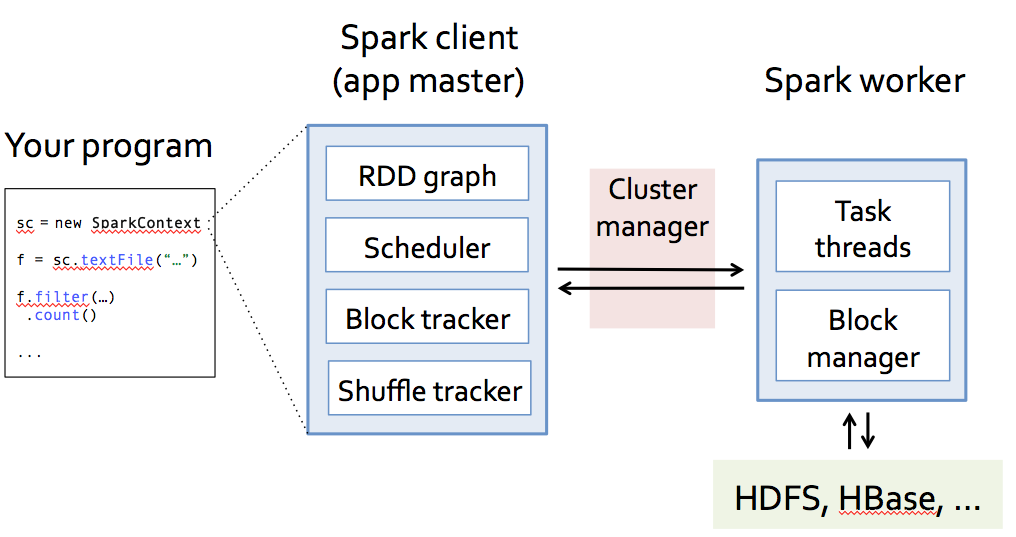
\includegraphics[scale=0.33]{./Figures/spark_components}
  \label{fig:spark_components_details}
\end{figure}
}

%%%%%%%%%%%%%%%%%%%%%%%%%%%%%%%%%%%%%%%%%%%%%%%%%%%%%%%%%%

% %%%%%%%%%%%%%%%%%%%%%%%%%%%%%%%%%%%%%%%%%%%%%%%%%%%%%%%%%%
\frame {\frametitle{In Summary}
% %%%%%%%%%%%%%%%%%%%%%%%%%%%%%%%%%%%%%%%%%%%%%%%%%%%%%%%%%%
\begin{itemize}
	\item {\bf Our example Application}: a \textbf{jar} file
	\begin{itemize}
		\item Creates a \texttt{SparkContext}, which is the core component of the driver
		\item Creates an input RDD, from a file in HDFS
		\item Manipulates the input RDD by applying a \texttt{filter(f: T => Boolean)} transformation
		\item Invokes the action \texttt{count()} on the transformed RDD
	\end{itemize}

	\item {\bf The DAG Scheduler}
	\begin{itemize}
		\item Gets: RDDs, functions to run on each partition and a listener for results
		\item Builds \emph{Stages} of \emph{Tasks} objects (code + preferred location)
		\item Submits Tasks to the \textbf{Task Scheduler} as ready
		\item Resubmits failed \emph{Stages}
	\end{itemize}

	\item {\bf The Task Scheduler}
	\begin{itemize}
		\item Launches \emph{Tasks} on executors
		\item Relaunches failed \emph{Tasks}
		\item Reports to the DAG Scheduler
	\end{itemize}

\end{itemize}

}
